\documentclass{article}
\usepackage{graphicx}
\usepackage{amsmath}
\usepackage{amsthm}
\usepackage{authblk}
\usepackage{listings}
\usepackage{amsfonts}
\newtheorem*{remark}{Remark}
\newtheorem{definition}{Definition}

\begin{document}

\title{Predicting Donald Trump's Tweets}
\author[1]{Adam Blakney}%\thanks{Email: akblakney@gmail.com}}
\date{}%21 Januari 2010\\\small{(Edisi Revisi : 3 Januari 2019)}}
\maketitle

\begin{abstract}
In this paper we apply several statistical learning, modeling,
and forecasting techniques to the problem of predicting the number of tweets Donald Trump will post in
a certain amount of time. We tailor our approach to the constraings of PredictIt's Tweet markets.
\end{abstract}

\section{Introduction}
Prediction markets are markets that allow users to bet on the occurence of events in the future ~\cite{def}.
In particular,
prediction markets may offer the opportunity to speculate about the outcomes of sports games, election outcomes,
etc. PredictIt is one such prediction market that focuses on political events~\cite{predictit}.
In particular, PredictIt offers markets that allow users to speculate on the number of tweets that certain
political figures will post in a pre-determined amount of time. Many different factors may be considered
in the task of predicting the Twitter behavior of a political figure; past Twitter behavior, current political
climate, and other current events may be relevant. In this paper, we focus on the use of past Twitter behavior
to predict future Twitter behavior. In particular, using the past Twitter behavior of the user
\lstinline{@realDonaldTrump} (see ~\cite{trump}) we aim to predict how many tweets
\lstinline{@realDonaldTrump} will post in time spans ranging from twelve hours to one week.

\section{PredictIt Tweet Markets}
In this section we give an brief overview of PredictIt's twitter markets, as well as a basic review of prediction markets.~\cite{def} and ~\cite{trading}
should be consulted for further information on prediction markets and trading.

\subsection{Markets, Brackets and Shares}
A market is composed of brackets, which specify possible market outcomes. Users interact with the market by buying ``Yes'' or ``No''
shares in each bracket, each of which is priced between \$.01 and \$.99. When the market resolves, exactly one bracket will resolve as the winning bracket while all others resolve as losing brackets.
At market closure, a winning bracket's ``Yes'' shares will be worth \$1; similarly a losing bracket's ``No'' shares will be worth \$1.
Thus, generally speaking, a user is incentivized to buy ``Yes'' shares in brackets they believe will win and ``No'' shares in brackets
they believe will lose.

\subsection{Maximizing Profit: Probabilistic Interpratation}
While the specifics of trading shares are rather involved (see ~\cite{trading}), here we discuss some basic facts about prediction markets, and explore
how one might profit off of miscalibrated markets. Specifically, in this section, we formalize the notion of expected profit and provide a framework for
interpreting prediction markets probabilistically. To formalize these concepts we first introduce the following definitions.
\begin{definition}
    A market $M$ is a collection of $n$ brackets, denoted $b_1,...,b_n$, one of which will resolve as the winning bracket, and the rest of which will
    resolve as losing brackets. The index of the winning bracket is unknown until the market closure.
\end{definition}

\begin{definition}
    For each bracket $b_i$, denote the ``Yes'' price by $s_i$, and denote the probability of it resolving as the winning bracket $p_i$.
    (Consequently, the probability of it resolving as a losing bracket is $1 - p_i$).
\end{definition}
Clearly, the probabilities $p_1,...,p_n$ are unkown: otherwise, assuming a rational market, the share prices $s_1,...,s_n$ would converge to them
and the market could not be exploited.
We now consider the impact of buying ``Yes'' or ``No'' shares in a market.
\begin{definition}
    Define $w_i$ to be the expected profit after buying one ``Yes'' share in bracket i and $\bar{w}_i$ to be the expccted profit after
    buying one ``No'' share in bracket i. Then,
    \begin{align*}
        w_i = .9p_i - s_i,
    \end{align*}
    \noindent and,
    \begin{align*}
        \bar{w}_i = .9(1-p_i) - (1-s_i),
    \end{align*}
\end{definition}
\noindent where the factor of $.9$ arises because PredictIt takes $10\%$ of profits.
Thus we note the following:
\begin{remark}
It is profitable to to buy a ``Yes'' or ``No'' share for bracket
$b_i$ when,
\begin{align*}
    .9p_i > s_i,
\end{align*}
\noindent or,
\begin{align*}
    .9(1-p_i) > 1- s_i,
\end{align*}
\noindent respectively.
\end{remark}
Thus, our goal is to estimate the probabilities $p_1,...,p_n$ reliably.

\subsection{\lstinline{@realDonaldTrump} Market Example}
For each selected Twitter user,
a new market is opened each week, and the market brackets---which users may place bets
on---are associated with the number of tweets to be posted by the account over that week.
Fig.\ref{market_graphic} shows a snapshot of a \lstinline{@realDonaldTrump} Twitter market.
The left-hand side gives the bracket outcomes, which specify the number of tweets to be posted by the user. Also visible
in the left-hand side is the users' stake in each bracket. Numbers boxed in green signify stake in a "yes" contract while
those in red signify stake in a "no" contract. For example, we see that in Fig.~\ref{market_graphic}, under the bracket title "220 - 229" is
the number 100 boxed in green, indicating that the user has stake in 100 "yes" contracts for the aformentioned bracket.
The remaining columns give market prices.
Note that we may interpret these market prices probabilistically. For example, consider 

\begin{figure}[h!]
    \centering
    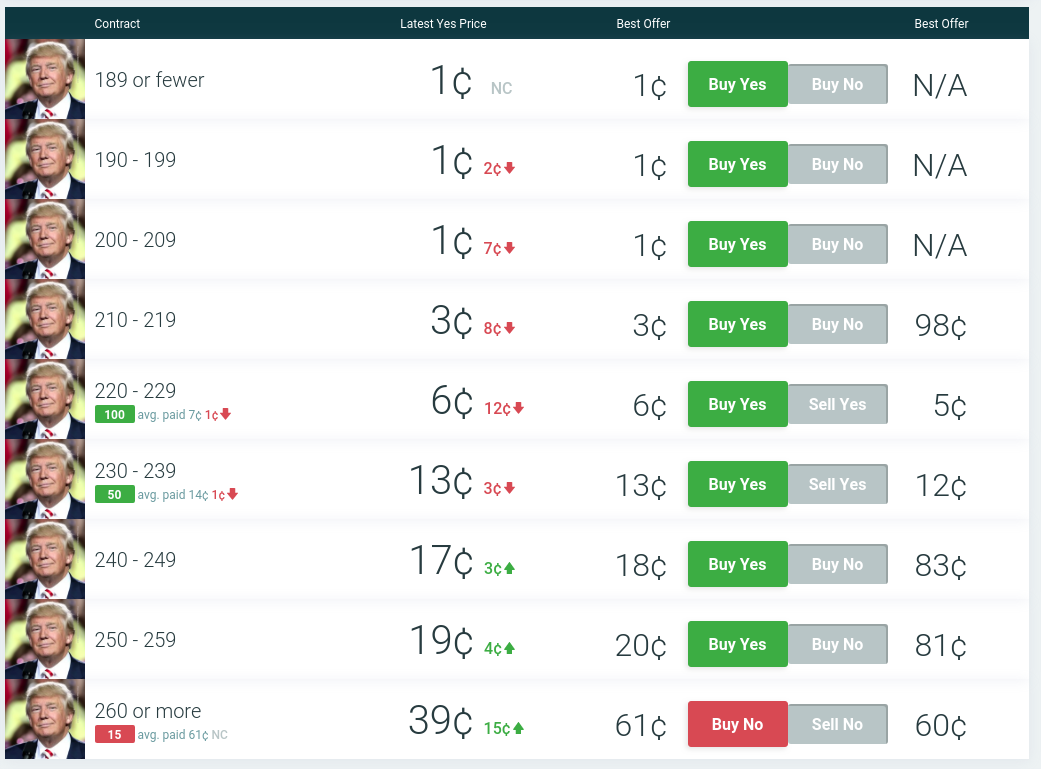
\includegraphics[width=1.0\textwidth]{market}
    \caption{A snapshot of the \lstinline{@realDonaldTrump} Twitter market with a users' stakes in various brackets.}
    \label{market_graphic}
\end{figure}

\section{Problem Formulation}
Recall that our goal is to estimate the probabilities $p_1,...,p_n$ of each bracket resolving as the winning bracket. More specifically,
we wish to predict the probability distribution of the number of tweets posted through the end of one week. To do so,
we model the history of tweet counts as outcomes of random variables, and use the observed
values to estimate the next random variable in the sequence.

Consider a continuous time interval of length $L$ partitioned into $N$ sub-intervals
$\tau_1,...,\tau_N$ each of length $l$ (in our case, $L$ is one week). Then we model the number of tweets during each of these intervals
as a random variable $X \in \mathbb{R}^N$, with,
\begin{align*}
\begin{pmatrix}
    X_1\\ \vdots \\X_N
\end{pmatrix}  &= 
\begin{pmatrix}
    \text{number of tweets during } \tau_1
    \\ \vdots \\
    \text{number of tweets during } \tau_N
\end{pmatrix}.
\end{align*}
Thus $\sum_{i=1}^N X_i$ gives the tweet count for the week associated with $X$.

Given a collection of random variables $X^{(1)},...,X^{(W)}$ representing tweet counts through $W$ weeks, our goal is to estimate
the distribution of $\sum_{i=1}^n X_i^{(W+1)}$ which gives the number of tweets during the next week.
%\begin{align*}

%\end{align*}

\subsection{Monte Carlo Simulation}
In this section we attempt to estimate the probabilities $p_1,...,p_n$ via Monte Carlo simulation.
We assume that the account's behavior is similar during similar times of the week. Thus, given $W$ weeks of data,
we partition each week into $N$ equal length intervals,
and track the number of tweets during each of these.
Consider the $W \times N$ matrix of previous tweet counts
$X$, where $X_{ij}$ gives the number of tweets during the $j$-th segment of the $i$-th. Given $X$, our goal, then,
is to estimate the distribution of $\hat{X}_{W+1} :=  (\hat{X}_{W+1,1},...,\hat{X}_{W+1,N})$ which gives the number of tweets during each of the $N$ segments
of the subsequent week. Then the estimate of the desired distribution is given by, $\sum_{j=1}^N \hat{X}_{W+1, j}$. 

\bibliography{mybib} 
\bibliographystyle{plain}


\end{document}